\documentclass{beamer}
\graphicspath{ {graphics/}}

\begin{document}
\title{Literary Worlds Javascript Client}
\author{John Lewis, Owen Watson, Tim Cunningham}
\usenavigationsymbolstemplate{}
\frame{\titlepage}
\frame{\frametitle{Table of contents}\tableofcontents}

\section{Background}
\frame{\frametitle{Background}
\begin{itemize}
  \item Literary Worlds is an multiuser text based game used for English education at WMU.
  \item These games are known as MOOs (Multiuser Object Oriented), or MUDs (Multi User Domains)
  \item Most of these games provide a telnet interface for playing, Literary Worlds uses enCore with MOOTcan, a Java applet.
  \item The aim of this project is to provide a drop-in replacement user interface in Javascript.
\end{itemize}
}

% - Title Page
% - Abstract
% - TOC
% - Intro
% - Background
% - Design Decisions
% - Stories
% - Implementation
%   - Continuous Integration - Tim
% - Testing
%   - Owen
% - Security
%   - Telnet is insecure
%   - Contain telnet in docker or similar
% - References
% - Glossary

\section{Introduction}
\frame{\frametitle{Introduction}
  \begin{itemize}
    \item LambdaMOO is distributed as a source tarball, deploying it on a new sever entails compiling it, and running it using the enCore database.

    \item enCore is an graphical interface and MUD database package that works with a LambdaMOO server to provide a browser based text client as well as a graphical, mouse driven interface.
    \item The Java applet is the text interface, it makes a telnet to LambdaMOO, as though the user were using a command line telnet client.
  \end{itemize}
}


\section{Xpress interface}
\frame{\frametitle{enCore Xpress interface}
  \begin{centering}
  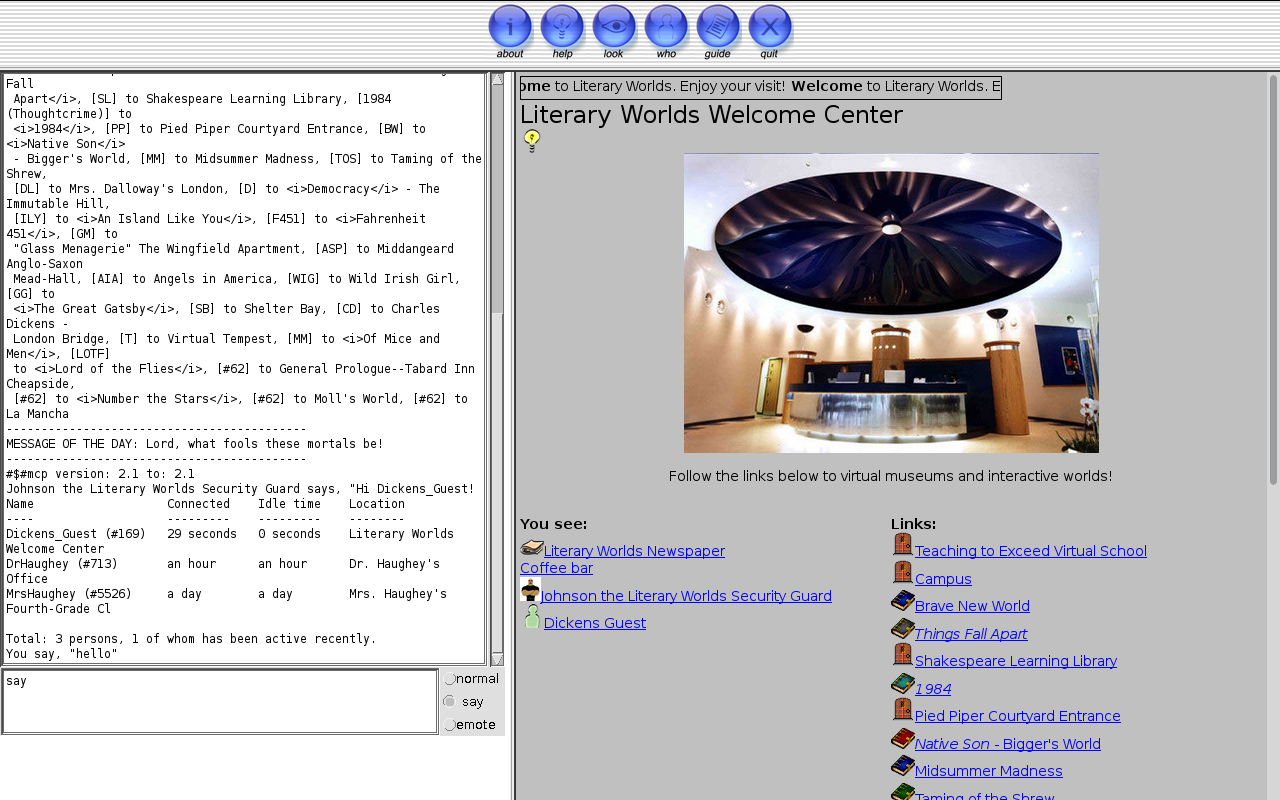
\includegraphics[width=\textwidth,height=\textheight,keepaspectratio]{classUsage.png}
  \end{centering}
}

\section{Design Decisions}
\frame{\frametitle{Client-Server Design}
  \begin{itemize}
    \item It is not possible to initiate a raw TCP connection in clientside Javascript, unlike Java applets.

    \item Therefore, we need an intermediary server to connect over TCP, as well as to the browser client, and send data back and forth between the two.

    \item This server must also support multiple concurrent users and handle asynchronous tasks and events.
  \end{itemize}
}

\frame{\frametitle{Client-Server Diagram}
}

\frame{\frametitle{Client Technology}
  % Backbone, Bootstrap, Socket.io, Coffeescript
  \begin{itemize}
  \item Socket.io
    \begin{itemize}
      \item Allows realtime communication between a server program and browser clients.
    \end{itemize}
  \item Backbone
    \begin{itemize}
      \item Backbone is a templating library for Javascript web applications
    \end{itemize}
  \item Bootstrap
    \begin{itemize}
    \item Bootstrap is a frontend layout toolkit
    \end{itemize}
  \item Coffeescript
    \begin{itemize}
      \item Coffeescript is a simple language that translates to Javascript
    \end{itemize}
  \end{itemize}
}

\frame{\frametitle{Server Technology}
  % Node.JS here
  \begin{itemize}
  \item Node.js
    \begin{itemize}
      \item Node.js is a server side runtime that uses the asynchronous features of Javascript to build web application servers. It provides a rich set of networking libraries, and uses the Google Chrome Javascript engine, V8.
      \item It is the first class citizen for socket.io, so it was natural to choose it for the server.
    \end{itemize}
  \item Express
    \begin{itemize}
      \item Express is a web app framework for Node.js
    \end{itemize}
  \end{itemize}
}


\section{Stories}
\frame{\frametitle{Stories}
  \begin{itemize}
  \item Text Mode
    \begin{itemize}
      \item Text
    \end{itemize}
  \item Graphical Mode
    \begin{itemize}
      \item Serving enCore GUI
    \end{itemize}
  \end{itemize}
}

\section{Implementation}
\frame{\frametitle{Continuous Integration}
\begin{itemize}
  \item Purpose
  \begin{itemize}
    \item Continuous integration aims to merge code from a developer's working copy many times a day into a shared mainline.
    \item Before any code is merged a, build server runs unit tests on the code, and if passed will be merged into the mainline.f
    \item This helps to improve the quality of the software and reduce the time to deliver it.
    \item The end goal of this process is to be able to automatically build and deploy the software whenever all of the tests are passing
  \end{itemize}
  \item Tools
\end{itemize}
}

\frame{\frametitle{Jenkins}
  \begin{itemize}
    \item Pros:
    \begin{itemize}
      \item Widely used and documented
      \item open sourced
      \item Wide range of support for different systems
      \item Can be extended with plugins
      \item Github integration
    \end{itemize}
    \item Cons:
    \begin{itemize}
      \item Manual setup required
      \item Have to get a server to run Jenkins
    \end{itemize}
  \end{itemize}
}

\section{Testing}
\frame{\frametitle{Unit Testing}
  \begin{itemize}
    \item Framework
    \item Matching Tools
  \end{itemize}
}

\section{Security}
\frame{\frametitle{Security}
  \begin{itemize}
    \item Telnet is plain text TCP, so it is inherently insecure to eavesdropping.
    \item In the future, the telnet server can be protected from external network using containerization such as docker
    \item This way only the Node.js server can connect via telnet, and user data can be protected with SSL in transport.
  \end{itemize}
}

\end{document}
